% This file was created with tikzplotlib v0.10.1.
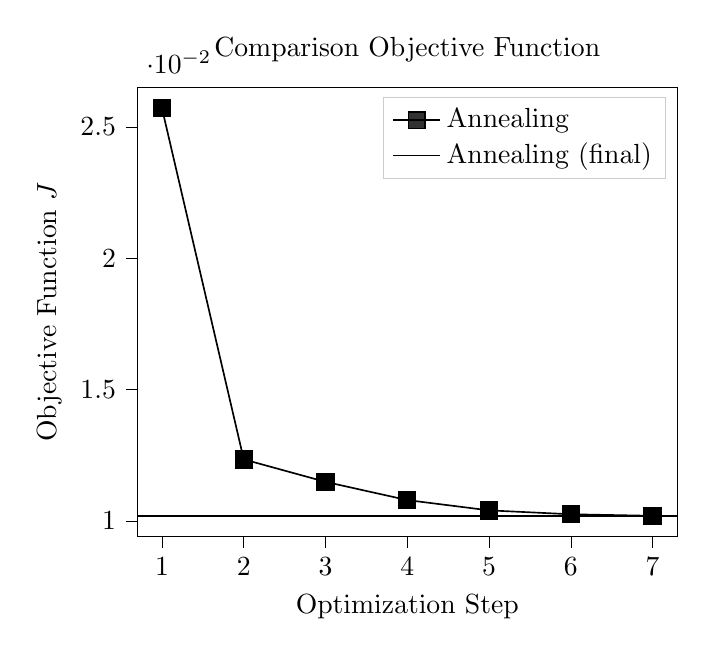
\begin{tikzpicture}

\definecolor{darkgray176}{RGB}{176,176,176}
\definecolor{lightgray204}{RGB}{204,204,204}

\begin{axis}[
legend cell align={left},
legend style={fill opacity=0.8, draw opacity=1, text opacity=1, draw=lightgray204},
tick align=outside,
tick pos=left,
title={Comparison Objective Function},
x grid style={darkgray176},
xlabel={Optimization Step},
xmin=0.7, xmax=7.3,
xtick style={color=black},
y grid style={darkgray176},
ylabel={Objective Function \(\displaystyle J\)},
ymin=0.00941407719526168, ymax=0.0264910506901239,
ytick style={color=black}
]
\addplot [semithick, black, mark=square*, mark size=3, mark options={solid}]
table {%
1 0.0257148246221756
2 0.0123398509201922
3 0.0114839448214397
4 0.010789879492589
5 0.0103977691960828
6 0.0102493034877965
7 0.01019030326321
};
\addlegendentry{Annealing}
\addplot [semithick, black]
table {%
0.7 0.01019030326321
7.3 0.01019030326321
};
\addlegendentry{Annealing (final)}
\end{axis}

\end{tikzpicture}
